\section{Results}

%TODO: use the definitions from definitions.tex

\paragraph{}
We investigated the relationship between entropy and cache traces, attempting to relate it to the cachability or prefetchability of a given trace.  What we found across several real-world traces is that distinct items are repeated very few times, making them poor predictors of what would be accessed next.  However, the differences between consecutive accesses (strides) are much more predictable.  While this predictability doesn't indicate that a trace will perform better in a cache on its own, it does indicate that a cache running the trace would greatly benefit from a prefetcher that can use stride data to predict the next access.

The predictability of the strides is evident in both the distribution of strides overall and by using conditional entropy measurements.  On any of the traces we tested, the distribution of strides is heavy-headed, leading to a lower entropy value than if the distribution was uniform.  This difference is consistently 2-5 bits of entropy for traces of all sizes (on the order of 1000-1000000 accesses) (Fig. \ref{fig:expected}).

\begin{figure}[ht]
    \centering
    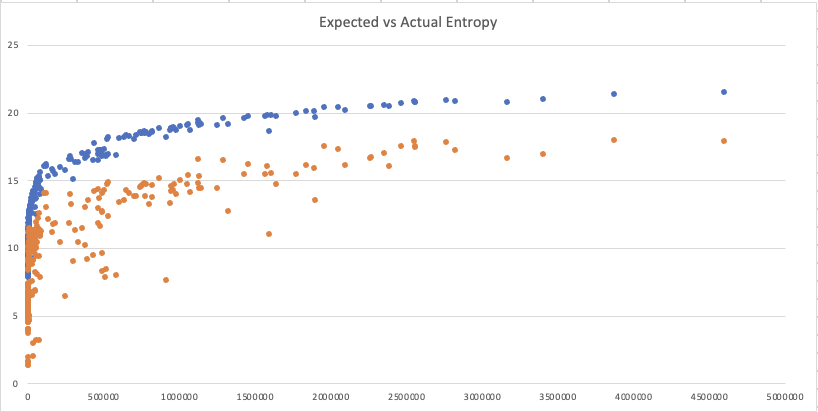
\includegraphics[scale=0.7]{expected entropy.png}
    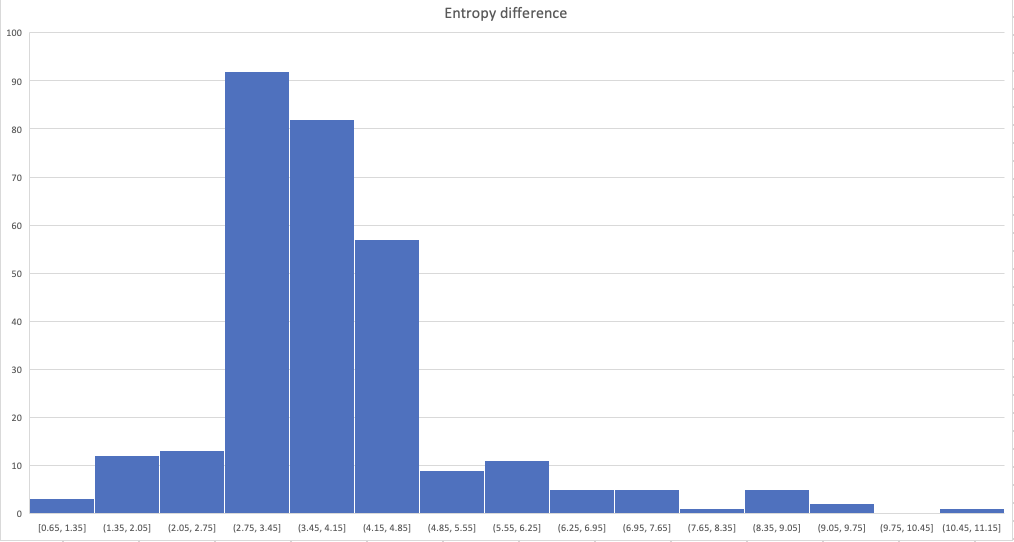
\includegraphics[scale=0.7]{entropy diff.png}
    \caption{Expected entropy (blue) and actual entropy (orange) plotted against trace length, and a histogram of the differences.  Expected entropy is calculated as the entropy if the strides are uniformly distributed.}
    \label{fig:expected}
\end{figure}
\newpage

%TODO: entropy notation is bad, should fix
We also measured the $n$-stride entropy $H_{s^n}(\sigma)$.  When $N = 1$, it stayed consistently below 5 bits, with an average of 2.37 bits, indicating a high degree of predictability (Fig.\ref{fig:cond1}).  As $N$ increases, the entropy falls off quickly, in part due to a lack of sample size.  For $N = 2$, most traces have $n$-stride entropy below 1.5 bits, with the average being about 0.7 bits (Fig.\ref{fig:cond2}).  Higher values of $N$ offer very little improvement to this value, and the conditions are repeated so rarely at $N = 3$ or higher that the $n$-stride entropy is measured as close to 0 due to a lack of samples.  However, the sample size for $N = 2$ may be large enough to conclude that it offers significant improvement over $N = 1$.

\begin{figure}[ht]
    \centering
    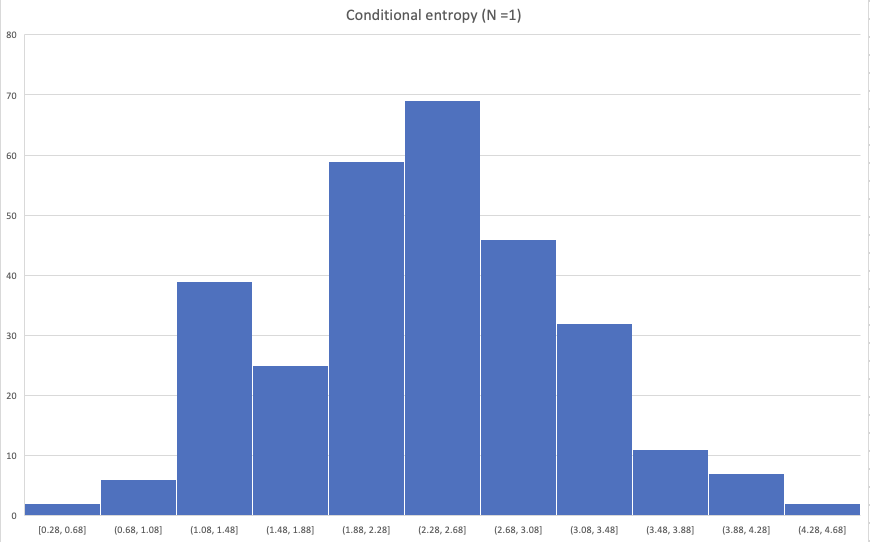
\includegraphics[scale=0.7]{conditional 1.png}
    \caption{Histogram of the conditional entropy when $N = 1$}
    \label{fig:cond1}
\end{figure}

\begin{figure}[ht]
    \centering
    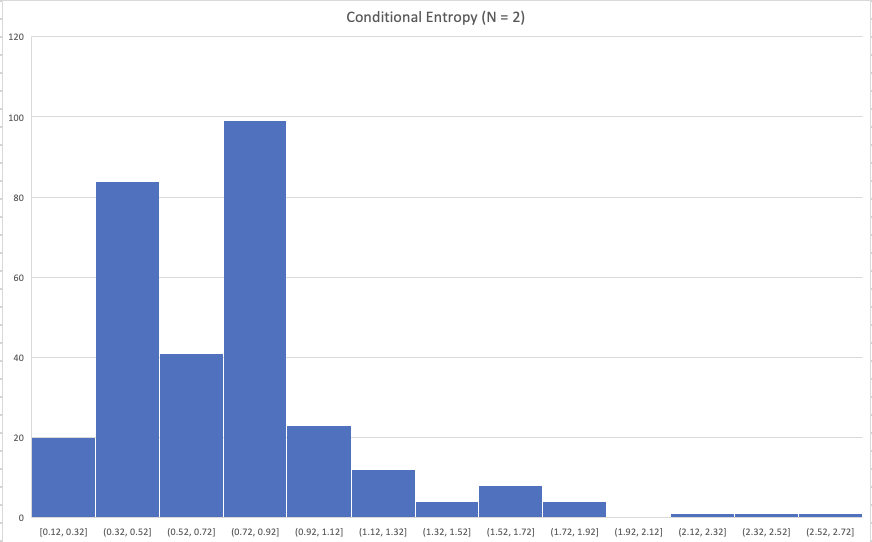
\includegraphics[scale=0.7]{conditional 2.png}
    \caption{Histogram of the conditional entropy when $N = 1$}
    \label{fig:cond2}
\end{figure}

These results indicate that it could be worthwhile to give a prefetcher the resources to perform irregular stride prefetching on the last two strides, or even the last one stride as that also provided a degree of predictability.  Additionally, we believe that these measures could be used to quantify the predictability (and prefetchability) of a specific trace.

We did not have conclusive results when calculating entropy on items as our data did not repeat items enough to provide a reasonable sample size.

%Importantly, stride entropy will always be higher than n-gram entropy, but takes less resources to do and collects data faster.  One of the insights from the n-gram entropy being low as a result of few repetitions is that keeping track of n-grams requires far more data to have a clear picture of the distribution, and gains are made by keeping track of strides, a more compact distribution.  Also, strides are relevant even when seeing new requests, where n-grams will always fail.
